\documentclass{abnt}

\usepackage[brazil]{babel}

\usepackage{geometry}                % See geometry.pdf to learn the layout options. There are lots.
%\geometry{landscape}                % Activate for for rotated page geometry
%\usepackage[parfill]{parskip}    % Activate to begin paragraphs with an empty line rather than an indent
\usepackage[utf8]{inputenc}
\usepackage{graphicx}
\usepackage{amssymb}
\usepackage{epstopdf}
%\usepackage{natbib}
\usepackage{url}
%\usepackage{abntcite}

% Formatação de código fonte - chupado descaradamente de http://www.kronto.org/thesis/tips/listings.html
\newenvironment{mylisting}
{\begin{list}{}{\setlength{\leftmargin}{1em}}\item\scriptsize\bfseries}
{\end{list}}

\newenvironment{mytinylisting}
{\begin{list}{}{\setlength{\leftmargin}{1em}}\item\tiny\bfseries}
{\end{list}}


\DeclareGraphicsRule{.tif}{png}{.png}{`convert #1 `dirname #1`/`basename #1 .tif`.png}

\titulo{Uma Plataforma de Software para o Estudo Interativo de Métodos e Algoritmos Econométricos}
\autor{Carlos Duarte do Nascimento}
\orientador{Professor Doutor Cicely Moitinho Amaral}
\comentario{Projeto e desenvolvimento de uma plataforma de software que permita o cadastro e a manipulação de procedimentos utilizados na econometria e implementações de metodos numéricos relacionados; Teste de um exemplo usando métodos numéricos em Econometria.}
\instituicao{Universidade de São Paulo}
\local{São Paulo}
\data{2008} 
 %\date{}                                           % Activate to display a given date or no date

\begin{document}
\folhaderosto
% Deve ser adicionado ao contador de pginas um, referente a folha de rosto.
% Obs.: A folha de aprovao no recebe nmero, nem  contada.
\addtocounter{page}{1}

%%%%%%%% RESUMO %%%%%%%%
\pretextualchapter{Resumo}
\vspace{4cm}
Propõe uma plataforma de \textit{software} cujo objetivo é servir de ao ensino de tópicos de Econometria. Trabalha um problema de Econometria apresentando métodos numéricos para a sua resolução. Descreve a experiência de implementar a plataforma e o problema proposto, comentando os resultados.


\newpage




% ************ SUMRIO ************
\sumario
%\section{}
%\subsection{}

\chapter{Introdução}

\section{Econometria: Teoria e Prática}

Dentre os objetivos de um curso de Econometria de nivel superior está a capacitação do aluno para compreender, construir e analisar modelos econométricos, utilizando-os como ferramentas para o planejamento estratético e a tomada de decisões relacionadas aos fenômenos estudados nestes modelos.

Neste sentido, é importante que o aluno tenha conhecimento tanto da teoria econômica envolvida quanto do instrumental matemático necessário para a modelagem dos fenômenos analisados. Esta meta só pode ser atingida se, aliada a uma sólida base teórica, o aluno puder interagir com estes modelos, realizando experiências e comparando resultados.

Tradicionalmente os cursos expoem o aluno a um pacote de software especializado, tal como o \em{EViews} ou o \em{SPSS}\footnote{Uma lista completa e atualizada de pacotes do gênero está disponível em \cite{web:econsoftware}}. Esta abordagem tem como principal vantagem a capacitação do aluno em uma ferramenta que ele possivelmente irá usar no seu dia-a-dia. 

Não é por acaso que tais ferramentas são adotadas universalmente por econometristas profissionais: elas automatizam muitos dos processos algébricos (regressões, aproximações numéricas) e estatísticos (testes de hipóteses, cálculo de estimadores qualitativos) envolvidos na modelagem econométrica. Entretanto, é exatamente este poder de simplificação que cria barreiras para o uso didático das mesmas: por mais importante que seja a visão geral do processo, a formação do aluno fica prejudicada se ele não é exposto aos detalhes computacionais do processo.

No extremo oposto, há professores que preferem o uso de um ambiente de programação tradicional, levando o aluno a construir suas próprias ferramentas e apresentar seus resultados na forma de "exercícios-programa". Esta abordagem permite maior aprofundamento, mas há a questão do tempo (a programação de um algoritmo de regressão simples, por exemplo, pode consumir boa parte do tempo de um curso básico de séries de tempo, por exemplo) e do interesse do aluno (que não pretende necessariamente se tornar um programador, mas apenas compreender a lógica do processo).

Estas duas abordagens nos levaram a experimentar uma alternativa intermediária: um sistema no qual um professor poderia mesclar textos teóricos com implementações de algoritmos para a resolução de problemas econométricos pontuais. O aluno poderia controlar seu nível de interação, podendo executar os algoritmos com dados pré-cadastrados, alterar estes dados e comparar os resultados, ou até mesmo criar seus próprios dados e sugerir mudanças nos algoritmos (caso tenha o conhecimento de programação de computadores para tanto).

\section {Um Problema Econométrico}

Seria difícil avaliar a eficácia da plataforma de software sem a implementação de um exemplo prático, o que nos leva a trabalhar nela um modelo econométrico de interesse e um instrumental matemático associado. Este capítulo aborda os detalhes matemáticos destas escolhas.

Judge, Griffiths, Hill e Lütkepohl\cite{judge} apresentam de forma sucinta e didática o uso de métodos numéricos de otimização para a estimação de parâmetros em modelos estatísticos no geral (tendo em vista os modelos econométricos apresentados ao longo do livro).

Para fins ilustrativos, eles resgatam um problema de [FALAR COM PROF. CICELY, é referenciado na pág. 956, mas não tenho a nota bibliográfica], que considera o modelo estatístico não-linear:

\[ y_t = \theta_1^* + \theta_2^* x_{t2} + (\theta_2^*)^2 x_{t3} +e_t , t = 1,2,...,20 \]
\[ y = f(\theta^*)+e\]

onde $y = (y_1, y_2, ..., y_{20})'$, $\theta^* = (\theta_1^*, \theta_2^*)'$ é o vetor de parâmetros, $e = (e_1, e_2, ..., e_{20})'$ e

\[ f(\theta)=
	\left( \begin{array}{ccc}
\theta1 + \theta_2 x_{12} + \theta_2^2 x_{13} \\
\theta1 + \theta_2 x_{22} + \theta_2^2 x_{23} \\
.\\
.\\
.\\
\theta1 + \theta_2 x_{20,2} + \theta_2^2 x_{20,3} \\


\end{array} \right)\
 \]
 
 O objetivo é encontrar um estimador de mínimos quadrados para $\theta^*$, e para tanto devemos minimizar a função:
 
 \[ H(\theta) = [y - f(\theta)]'[y - f(\theta)] \]

Este é um problema econométrico típico, já adaptado a um modelo matemático, que se presta bem a ilustrar a aplicação de uma plataforma como a proposta, razão pela qual nos pautamos sobre ele.




\chapter {A Plataforma}

\section{Proposta Funcional}

O objetivo do sistema é facilitar o estudo de conceitos e técnicas de econometria. Suas principais áreas funcionais\footnote{Tais áreas estão propositalmente definidas de forma superficial, com o objetivo de não prjeudicar o caráter experimental do trabalho. Um produto de software mais objetivo deveria seguir a linha proposta por Jacobson\cite{Jacobson}.} seriam:

\subsection{Usuários}
O sistema irá identificar os usuários no sistema, qualificando-os entre aqueles que irão introduzir o material a ser trabalhado (doravante denominados \textit{professores}) e aqueles que irão trabalhar este material (que chamaremos de \textit{alunos}).
\subsection{Aulas}
A introdução do material didático no sistema é feita pelo professor. Para fins de organização, cada tópico abordado será tratado como uma \textit{aula}, dividida em um ou mais \textit{passos}, que serão apresentados sequencialmente ao aluno quando ele selecionar uma determinada aula.

Cada passo da aula consiste em:
\begin{itemize}
\item Parte teórica: Conteúdo textual/HTML simples, explicando o que será executado; 
\item Parte prática: Abaixo do texto teórico, o aluno encontrará campos onde poderá entrar com dados e executar um código previamente preparado pelo professor, obtendo resultados imediatamente. Esta execução pode ser feita repetidas vezes, variando os dados ou mesmo observando múltiplas iterações de um determinado algoritmo, até que o aluno decida avançar para o passo seguinte.
\end{itemize}

Desta forma, o professor pode programar possibilidades experimentais para o aluno, tornando o experimento tão amplo quanto deseje. É necessário codificar apenas a parte matemática/econométrica (muitas vezes já praticamente pronta na literatura) - sendo que a plataforma irá cuidar dos detalhes relacionados a compilação, fluxo e apresentação ao aluno.

Para o aluno tudo fica simplificado também - não há exposição ao código, apenas ao texto e à ferramenta para experimentar. Uma possibilidade é salvar os dados de entrada/saída para uso futuro (ou para avaliação do professor). Também é interessante que o aluno possa carregar dados pré-existentes disponibilizados pelo professor (por exemplo, dados reais aplicados em um modelo).


\section {Modelagem}

\subsection{Diagrama de Classes de Entidade}
As principais entidades são modeladas de acordo com o diagrama na Figura \ref{classes}.

\begin{figure}
\begin{center}
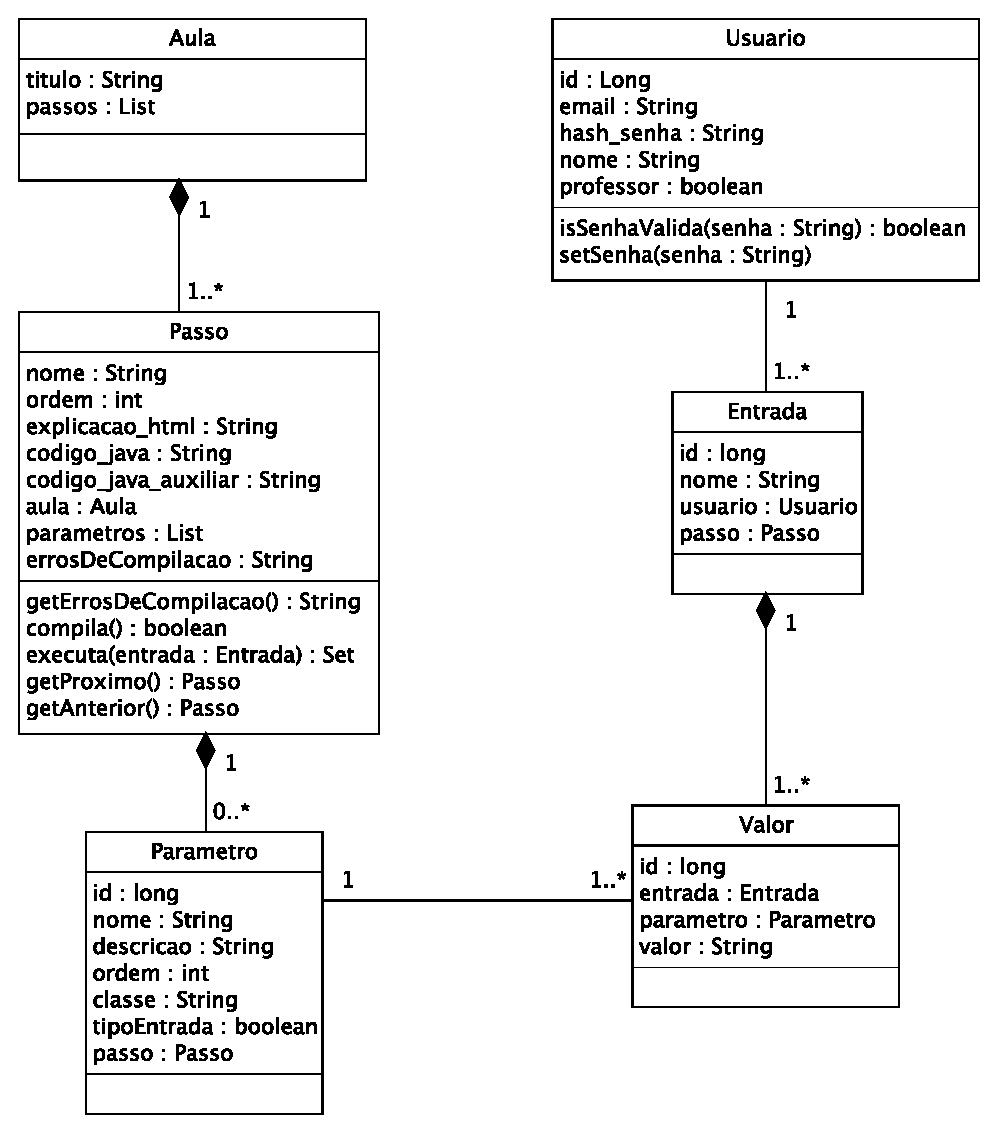
\includegraphics[scale=0.8]{classes.eps}
\caption{{\bf Classes de Entidade do Sistema}}
\label{classes}
\end{center}
\end{figure}

\textbf{Passo} é a entidade mais importante do sistema, representando cada tela com a qual o usuário interage, incluindo o código-fonte (algoritmo) que será experimentado pelo aluno. Uma \textbf{Aula} agrupa um conjunto de passos, permitindo a organização do conteúdo didático.

Cada variável que o professor determina que o aluno poderá inserir ou recuperar de um passo é um \textbf{Parametro}. Os dados efetivamente entrados pelo aluno são representados por objetos \textbf{Valor} e guardados coletivamente na forma de \textbf{Entrada}.

\subsection{Casos de Uso}

No geral, as iterações mais importantes do sistema são os casos de uso apresentados na Figura \ref{casos}, cujos passos são descritos\footnote{Tradicionalmente, Casos de Uso são descritos através de vários campos-padrão (nome, atores, pré-requisitos, passos, etc.), seguindo as linhas gerais delineadas por Jacobson\cite{Jacobson}. Tendo em vista o foco do trabalho, optamos por uma descrição mais sucinta, focada nos passos e em linguagem natural} em seguida.

\begin{figure}[htbp]
\begin{center}
\includegraphics[scale=0.75]{casos.eps}
\caption{{\bf Casos de Uso do Sistema}}
\label{casos}
\end{center}
\end{figure}

\subsubsection{UC1. Criar Aula}
Após dividir o conteúdo didático em aula, o professor insere cada uma delas no sistema, atribuindo um nome e uma descrição breve.
\subsubsection{UC2. Adicionar Passo}
Cada aula é dividida pelo professor em um ou mais passos, que serão executados sequencialmente pelo aluno. Para cada passo adicionado, o professor dá um nome, cadastra um texto explicativo e um algoritmo que será executado como exercício ao final da leitura do texto, com parâmetros de entrada e saída também definidos pelo professor.
\subsubsection{UC3. Interagir com Aula}
Uma vez tendo o material preparado, o aluno pode entrar no sistema e visualizar a lista de todas as aulas. Ao selecionar uma delas, o primeiro passo tem seu texto explicativo exibido, e, ao final, o aluno pode entrar com os dados e verificar os resultados, como programado pelo professor.


Um projeto de software mais elaborado poderia documentar 
Para maior clareza, seguem algumas das páginas \footnote{Um projeto de software mais elaborado poderia documentar estas interações na forma de Casos de Uso UML\cite{}}

\chapter {Arquitetura de Software}



\section{Tecnologias}
Uma vez definida a funcionalidade desejada, faz-se necessário selecionar tecnologias (linguagens, ferramentas e frameworks) e metodologias (padrões de projeto) que facilitem a criação da plataforma de software desejada de forma eficiente, e, acima de tudo, de forma expansível para acomodar necessidades futuras.

As escolhas definidas aqui foram norteadas por dois pré requisitos: que todas as metodologias tenham referencial acadêmico e implementações bem-sucedidas; e que todas as ferramentas utilizadas sejam gratuitas e de código livre, garantindo que a aplicação  possa ser ampliada e modificada por qualquer entidade interessada, sem que hajam restrições de qualquer natureza.
\subsection{Linguagem de Programação}
É necessário fazer duas escolhas neste tópico: a da linguagem a ser utilizada para construir o aplicativo, e a da linguagem através da qual os algoritmos serão descritos para a mesma.

Para o aplicativo, é preciso ter uma linguagem que ofereça performance, escalabilidade, suporte ao desenvolvimento para a web e facilidade para trabalhar com bancos de dados relacionais (ferramenta indispensável para o volume de dados gerado pelo uso em larga escala, vide adiante). Também é importante que a linguagem não seja excessivamente obscura ou limitada a um nicho de mercado, já que um dos objetivos é propor uma plataforma que possa ser ampliada e melhorada por quem tenha interesse.

Já o algoritmo exige uma linguagem que possa ser compilada ou interpretada dinamicamente, que tenha respaldo acadêmico (para aproveitar o código e, mais importante, o conhecimento pré-existente no corpo docente) e, preferencialmente, que já possua um ambiente de compilação/runtime livre (a implementação de tal ambiente não as complexidades inerentes a este tipo de implementação fogem ao escopo deste trabalho). 

Com o uso dos mecanismos de arquitetura apropriados é possível trabalhar ambas as demandas através de uma linguagem única. Esta abordagem simplifica o projeto e reduz a barreira de entrada para novos desenvolvedores, e foi considerada antes de tentar trabalhar com uma linguagem de aplicação separada da linguagem de algoritmos.

Embora existam linguagens de domínio específico para algoritmos matemáticos, faz sentido considerar primeiro linguagens de uso geral (ainda no sentido de simplificar e popularizar a plataforma). Estudos como o de Prechelt\cite{Prechelt} abordam aspectos como tempo de desenvolvimento e performance para o uso geral, mas é necessário levar em conta as necessidades particulares desta aplicação. Isto nos levou a considerar:

\subsubsection{C/C++}
A melhor opção em termos de performance. Por ter acesso aos mais diferentes tipos de bilbiotecas nos diversos sistemas operacionais existentes, também não apresentaria problemas para trabalhar com banco de dados ou com web. No entanto, a programação nesta dupla é bastante sujeita a erros, e muitas vezes é preciso escolher entre a flexibilidade do C++ e a performance do C.

Além disso, é necessário um esforço extra para garantir a compabilidade entre diferentes plataformas. Tais fatores elevariam o tempo do  projeto e colocariam uma barreira à entrada de novos desenvolvedores – isso sem falar que dificilmente a programação dos algoritmos seria feita de forma didaticamente viável nela.

\subsubsection{Pascal}
Tem a seu favor um excelente balanço entre performance e facilidade de programação (por ser mais fortemente tipada do que C e executar muitas das verificações de erros comuns em tempo de execução), além de possuir extensões de orientação a objeto e implementações livres (como o Free Pascal). No entanto as universidades já não tem mais incluído esta linguagem em seus currículos (Java é o substituto mais comum), o que se reflete em reduzida disponibilidade de programadores.

\subsubsection{Fortran}
Um dos pontos fortes é a vasta quantidade de algoritmos matemáticos e estatísticos disponíveis na literatura já codificados nesta linguagem. No entanto, a linguagem oferece poucas facilidades para a programação na web, e a mão-de-obra disponível é muito limitada ao meio científico/acadêmico.

\subsubsection{Java (opção final)}
O equilíbrio entre as demandas funcionais e não-funcionais levou à escolha da linguagem Java para a primeira implementação. Estudos como o de Bull, Smith, Pottage e Freeman\cite{BullSmithPottageFreeman} mostram que apresenta performance comparável a C, aliada a uma ampla gama de bibliotecas/frameworks que tornarão a implementação mais simples e expansível.

Uma vantagem adicional é a possibilidade que a linguagem oferece (a partir da Versão 6) de que o compilador seja invocado através de APIs de alto nível, permitindo a execução interativa dos algoritmos econométricos de forma independente de sistema operacional ou plataforma.

Caso esta escolha não seja a mais apropriada no futuro, uma possibilidade que estará disponível são  linguagens dinâmicas como Ruby, Python ou LISP, ou, alternativamente, como linguagens estáticas com suporte a reflexão, como C\# ou Objective-C – observando-se o mapeamento dos mecanismos de arquitetura para recursos equivalentes em cada uma delas.

\subsection{Ambiente de Desenvolvimento, Compilação e Publicação}

É importante que o processo de compilação e publicação (\textit{deploy}) da aplicação sejam completamente automatizados, de forma que qualquer pessoa possa facilmente descarregar o código existente de um repositório, testá-lo e implementar novas características.

A grande quantidade de frameworks envolvidos no processo gera uma dificuldade adicional: o gerenciamento de dependências. Tento isto em vista, usaremos o Maven\footnote{\url{http://maven.apache.org}} não apenas para executar a compilação e publicação, mas também para recuperar automaticamente todas as bibliotecas (.JAR) de frameworks utilizados a partir da Internet.

O código-fonte não irá exigir nenhum IDE\footnote{\textit{Integrated Development Environment} - Ambiente de Desenvolvimento Integrado} em particular. No entanto, o Eclipse (\url{http://eclipse.org}) será utilizado como ferramenta base, sempre tomando o cuidado de não tornar a ferramenta dependente dele. 

\section{Testes Automatizados}

É muito importante que o sistema mantenha os resultados consistentes, mesmo com a implementação de novas funcionalidades. Para tanto, a criação de testes automáticos (unitários e funcionais) durante o processo de desenvolvimento (e não como um detalhe adicional) é desejável - de fato, autores como Janzen e Saiedian\cite{Janzen_Saiedian} defendem a idéia de que o desenvolvimento como um todo deve ser pensado com foco nos testes, alegando que esta abordagem (\textit{Test-Driven Development}) teria impacto positivo na qualidade do código gerado e do produto final.

Sistema Java costumam usar o framework JUnit\footnote{\url{http://junit.org}} para implementação de testes unitários automáticos, devido à sua natureza não-intrusiva (mantendo o código de testes separado do restante) e seu amplo leque de capacidades embutidas, mantendo o código de testes bastante sucinto. Mesmo testes funcionais automáticos podem ser feitos através dele (uma estratégia é expandi-lo através da extensão JFunc\footnote{\url{http://jfunc.sourceforge.net}}, desenhada para este fim).

\subsection{Padrões de Projeto}

Sob a perspectiva da arquitetura geral, o sistema pode ser visto como uma coleção interativa de CRUDs\footnote{\textit{Create-Read-Update-Delete}, acrônimo para módulos que efetuam estas quatro operações básicas sobre algum tipo de entidade -uma referência ao termo (contextualizada num ambiente OO) se encontra em Kilov\cite{kilov_crud}}. As exceções ficam por conta da execução interativa de algoritmos e da importação de dados), sendo, portanto, razoável trabalhar com a separação em três camadas descrita por Eckerson\cite{Eckerson1995}:

\begin{itemize}
\item Uma camada de interface (front-end), utilizando MVC e outros princípios detalhados a seguir.

\item Uma camada intermediária de “fachada”, agrupando as operações de alto nível. Esta será implementada parcialmente através do mecanismo de MVC e (onde o reuso justificar) em classes de apoio através de objetos simples\footnote{\textit{POJO}, isto é, Plain Old Java Objects};

\item Uma camada de operações (back-end) tais como: armazenamento de dados, execução de algoritmos e conversão de formatos, cuja implementação é detalhada adiante;


\end{itemize}

\begin{figure}[htbp]
\begin{center}
DESENHAR
\caption{Diagrama da Arquitetura}
\label{default}
\end{center}
\end{figure}


As melhores práticas de desenvolvimento de software muitas vezes demandam a implementação de diversos padrões de projeto\footnote{Dados empíricos mostram\cite{IeeeExperience} a relação entre este tipo de padrão e a qualidade do software}. Felizmente, a plataforma Java conta com diversos frameworks que implementam tais padrões de projeto, economizando esforço e tornando o código mais enxuto e focado no problema educacional.

O restante desta sessão é dedicado a descrever e justificar algumas destas práticas, definindo (quando aplicável) os frameworks selecionados para a implementação das mesmas.

\subsubsection{Mapeamento Objeto-Relacional}

Ao longo das últimas décadas, os sistemas gerenciadores de banco de dados relacionais (RDBMS)  simplificaram o armazenamento de dados através da introdução da abordagem relacional de representação dos mesmos, implementada em pacotes de software de baixo custo, de forma isolada da aplicação principal, permitindo ao desenvolvedor concentrar-se no domínio específico do problema computacional a ser resolvido\footnote{Para uma perspectiva histórica, consulte Codd\cite{Codd1970}}.

Além disso, a popularização dos RDBMS permitiu o uso de recursos computacionais relativamente limitados (tais como microcomputadores) para a execução de tarefas de manipulação de dados anteriormente restritas a sistemas de grande porte (e elevado custo de operação e manutenção), razão pela qual o uso de um RDBMS é indicado em qualquer sistema no qual a manipulação indireta dos dados não represente impacto na performance.

Tal característica, aliada à importância que os dados representam para as organizações (chegando, em muitos casos, a ser mais valiosos que os aplicativos ou os meios físicos nos quais eles são armazenados e processados), fez com que muitos dos sistemas desenvolvidos entre as décadas de 80 e 90 tivessem o modelo relacional de banco de dados como base do seu projeto – o software que manipularia estes dados era pensado de forma secundária, quase que conseqüência direta do desenho do banco.

Com a introdução das técnicas de desenvolvimento de software orientado a objeto – outro artefato que aumentou o nível de abstração com o qual os projetistas de software lidam com o domínio dos problemas (e, portanto, a sua produtividade) – surgiu uma nova abordagem: proponentes destas técnicas defendem que o sistema deve ser modelado sob o ponto de vista de suas classes – o armazenamento em meio não-volátil dos objetos destas classes (agora denominado \textit{persistência}) passa a ser visto apenas como uma capacidade adicional das mesmas, e o banco de dados torna-se um mero armazém de objetos\footnote{Uma descrição isenta de plataforma deste tipo de mapeamento é dada por Ambler\cite{web:ambler}}.

A plataforma proposta neste trabalho segue esta nova abordagem, para a qual se coloca um problema: como representar a riqueza gramatical dos elementos da orientação a objeto (tais como herança, polimorfismo e navegabilidade) dentro do sistema de modelagem relacional dos RDBMS? Esta questão se divide em dois aspectos: o da busca da metodologia para mapear estas características e o da forma de implementá-la (evitando a redundância de código).

Este problema não é novo\footnote{Kilov novamente}, tampouco exclusivo desta aplicação. A técnica para resolve-lo é denominada mapeamento objeto-relacional, e na plataforma Java existem diversos frameworks de código livre que a implementam\footnote{Uma lista ampla pode ser encontrada em \url{http://java-source.net/open-source/persistence}}. Neste caso uma análise mais aprofundada pôde ser dispensada, visto que o Hibernate\footnote{\url{http://www.hibernate.org}} é o padrão de facto adotado pela comunidade Java para sistemas com características de persistência convencionais, tais como este.

O Hibernate é um framework de código totalmente livre, que gera automaticamente e em tempo de execução as declarações SQL necessárias para persistir e recuperar objetos no RDBMS. O código SQL gerado é geralmente muito otimizado, e é possível customizar qualquer declaração que não seja aceitável. Além disso, a Versão 3 permite o uso de annotations, isto é, do desenho do mapeamento sobre o próprio código. Esta característica torna os arquivos de mapeamento (que usualmente demandam muito tempo e acrescentam um passo extra na compreensão do código) dispensáveis, o que, por si só, já justifica o seu uso.

Uma outra técnica para implementar o conceito de persistência é a chamada prevalência - nela, o estado dos objetos é armazenado em sistemas de arquivo tradicionais, num misto de serialização e de aualizações de estado (balanceando segurança dos dados e performance). Tal abordagem pode ser implementada usando um framework como Prevayler\footnote{\url{http://www.prevayler.org}} para adicionar a capacidade de prevalência às classes de domínio. Embora esta técnica simplifique o deploy por dispensar um SGBD, a quantidade de memória RAM necessária para manter todo o grafo de objetos em memória tornaria inviável o uso da aplicação em larga escala.

\subsubsection{Apresentação e MVC (Model / View / Controller)}

Devido à sua natureza de interação com o usuário, a camada de apresentação é uma das mais sujeitas a alterações. Além disso, seu fluxo pode se tornar bastante complexo, o que favorece a duplicação de código desnecessária.

O padrão de projeto Model/View/Controller (MVC) tem se demonstrado útil na redução destes problemas. Nele, a camada de apresentação é segregada em dois tipos de componentes: view (composta pelas diversas interfaces do sistema, e desprovida de qualquer código que não esteja relacionado à interação com o usuário e à pré-validação dos dados introduzidos por ele) e model (código que responde a ações imperativas do usuário, tais como submeter um formulário de dados ou solicitar uma funcionalidade).

View e Model operam de forma totalmente independente: componentes de model respondem às solicitações utilizando as camadas inferiores e retornando algum tipo de status (ex.: “sucesso”, “operação inválida”, etc.), e componentes de view apresentam dados anexados a eles e retornam os dados novos ou alterações feitas pelos usuários.

A conexão entre eles é feita pelo controller: um componente que, para cada solicitação da view, dispara um ou mais componentes do model, e, conforme o resultado, apresenta uma nova view. Todo o fluxo é mantido neste componente (no código ou em um arquivo de configuração), desacoplando o código e oferecendo uma visão de alto nível que torna fácil identificar componentes reutilizáveis e/ou o impacto de quaisquer mudanças\footnote{Tygre descreve sua primeira implementação de MVC na interface gráfica original da Xerox, mas a consolidação do modelo em sistemas web é atribuída a Gamma / Helm / Johnson / Vlissides\cite{Gamma1995}}.

Embora seja possível adotar a filosofia MVC através do desenvolvimento direto, muito trabalho pode ser popupado através do uso de um framework MVC que, dentre outras coisas, implemente um controller configurável e auxilie na passagem de dados entre model e view (tarefa que se torna complexa à medida em que se considera a generalidade do HTML no tocante a formulários de dados, e o desejo de usar técnicas como AJAX para aumentar a usabilidade da aplicação). De início, foram considerados os frameworks mais utilizados atualmente, a saber:

\begin{itemize}
\item Struts: Um dos frameworks mais tradicionais em Java, tem como vantagens uma biblioteca de apresentação bastante rica e evolução constante. Sua maior limitação é a grande quantidade de código/configuração necessários para definir o fluxo da aplicação;
\item Spring MVC: É parte do framework Spring, o que facilitaria a sua integração. Mas também sofre do mal de exigir muita configuração, sem apresentar maiores atrativos que compensem o fato;
\end{itemize}

Tendo em vista que as alternativas padrão não atendem às necessidades do projeto, pesquisamos frameworks com menor base de usuários, tais como VRaptor, Jaffa e Stripes. Este último, por contar com excelente documentação e muitos exemplos na web, foi escolhido para a implementação.

Finalmente, é importante salientar que existe uma outra alternativa para otimizar o desenvolvimento da camada de apresentação: o uso de arquiteturas baseadas em componentes, tais como Wicket, WebWorks e JSF (os dois primeiros são frameworks, o último é uma especificação para este tipo de arquitetura, definida sob supervisão da empresa que desenvolve o Java e seguida por diversos frameworks), sobretudo pela agilidade que oferecem na prototipação e na criação de interfaces. No entanto, aplicações desenvolvidas sob este tipo de arquitetura não possuem a “tolerância a mudanças” que o MVC proporciona (e estas mudanças seguramente ocorrerão à medida em que a plataforma for expandida), razão pela qual descartamos tal tipo de solução.

\subsubsection{Inversão de Controle / Injeção de Dependências}

Tendo em perspectiva que a aplicação resultante deste projeto será uma base para o desenvolvimento de outros sistemas, é importante que a mesma seja de fácil compreensão e manutenção.

Um dos grandes obstáculos para a manutenção de projetos de software é o acoplamento excessivo entre os seus diferentes módulos e camadas. Ainda que se use (e usamos) boas práticas de separação das mesmas (tais como a arquitetura Model-View-Controller e o modelo de três camadas), se estas camadas apresentarem excessiva dependência cruzada, pequenas alterações irão demandar grandes esforços de codificação e teste.

A inversão de controle\footnote{Fowler\cite{FowlerIoc} define a IoC como uma característica comum em frameworks, mas uma vez identificada, esta passou a ser usada como técnica de projeto } (IoC) é uma técnica de projeto que aborda o problema do acoplamento subvertendo a maneira tradicional com que um módulo do sistema solicita funcionalidade a outro módulo (daí o nome). O princípio fundamental é que um módulo que dependa de outro para executar a sua funcionalidade não o chama explicitamente – ao invés disso ele manifesta esta dependência de alguma forma, e o ambiente operacional cuida de oferecer o componente que melhor ofereça o tipo de serviço necessário.

Isso faz com que o módulo se concentre na sua própria funcionalidade – ao invés de misturar este código com o código que cuidará da iteração com a dependência. Há um ligeiro aumento na quantidade de código devido à necessidade de formalizar a dependência através de suas características (e não através da chamada direta do módulo que satisfaz a dependência) – o exemplo canônico de Fowler mostra essa diferença. Mas isto é largamente compensado pelo desacoplamento obtido, e a clareza do código não é prejudicada.

Existem várias formas de implementar o princípio de IoC, sendo que a Injeção de Dependências é bastante popular por reduzir a quantidade de código envolvida no processo\footnote{Fowler descreve esta implementação na forma de um padrão de projeto\cite{FowlerInjdep}}. Nela, o módulo que oferece a funcionalidade apresenta uma interface não apenas para as tradicionais chamadas, mas também para as dependências delas (ex.: conexões de banco de dados, canais de saída, etc.). O módulo que solicita a funcionalidade o faz como na programação tradicional (chamando o método exposto), mas um framework media estas chamadas e fornece as dependências necessárias de forma apropriada. O Spring\footnote{\url{http://www.springsource.org/}} tem se tornado um padrão no mundo Java para esta tarefa, a exemplo do que o Hibernate faz no mapeamento objeto-relacional. No entanto, isso deve ser balanceado com a real neceissade do sistema, evitando torná-lo mais complexo que o necessário.



%\section {Modelo Econométrico: Séries de Tempo}

%Séries de Tempo consistem em conjuntos de observações discretas de um fenômeno feitas ao longo de um período de tempo. Elas diferem de outros conjuntos de dados por apresentar dependências entre observações vizinhas, relações sazonais e outras caraterísticas únicas que podem ser aproveitadas na sua análise.

%Tal análise permite a criação de modelos que permitem a elaboração de previsões, que são do maior interesse para pesquisadores e para o público em geral. Exemplos econométricos característicos incluem a previsão do comportamento de ações em bolsas de valores\cite{wikipedia:time_series}, ou a determinação do impacto de fatores qualitativos em vendas de produtos.




\chapter{Resolução do Problema}



\section {Métodos de Gradiente}

O problema descrito anteriormente pode ser resolvido através de métodos de aplicados a problemas sem restrições. A proposta dos autores (pp. 951 -- 954) é trabalhar métodos iterativos, nos quais se busca uma seqüência de parâmetros $\theta_{1}, \theta_{2}, ... , \theta_{n}$ que minimizam a função-objetivo  $H(\theta)$.

Isto significa que, para cada iteração $n$, temos uma matriz de direção $P_{n}$ e tamanho de passo $t_{n}$, que multiplicados pelo gradiente da função H ($\gamma_{n}$) permitem determinar o parâmetro para o passo seguinte, isto é:

\[ \theta_{n+1} = \theta_{n} - t_{n}P_{n}\gamma_{n} \]

O método torna-se completo quando determinamos uma condição de parada. Idealmente o faríamos quando a função objetivo não puder mais ser minimizada. Para fins práticos, paramos quando a redução passar a ser insignificante, por exemplo, se, para um $\epsilon > 0$ suficientemente pequeno e um $l$ inteiro e positivo tivermos uma das seguintes condições:

\begin{enumerate}
\item $ ( \theta_{n+l} - \theta_n )'( \theta_{n+l} - \theta_n ) < \epsilon$
\item $ H(  \theta_n )- H (\theta_{n+l} ) < \epsilon$
\item $  [\frac{\delta H}{\delta \theta}\vert_{\theta_n}]'[\frac{\delta H}{\delta \theta}\vert_{\theta_n}] < \epsilon$
\end{enumerate}

Além disso, devemos impor limites no número de passos e/ou tempo de compilação, e tentar novos valores iniciais quando este tipo de condição ocorrer.

A diferença principal entre os vários métodos de gradiente se dá no critério para a escolha da direção do passo, isto é, da matriz de direções $P_n$.

A seguir apresentamos alguns métodos detalhados pelos autores, acompanhados do código Java correspondente. Estes trechos de código podem ser usados diretamente na construção de uma aula sobre o assunto na plataforma.

\subsection{Newton-Raphson}

Este algoritmo consiste em usar o inverso da matriz Heissiana para especificar a direção do passo em cada iteração, ajustando-o pelo gradiente, isto é:

\[ \theta_{n+1} = \theta_{n} - \mathcal{H}_{n}^{-1}\gamma_{n} \]

O código abaixo calcula, para um par \textit{theta1} / \textit{theta2}, a matriz com o passo, isto é, os valores que, subtraídos deste par, resultarão no par correspondente ao passo seguinte\footnote{O código da função hess, que calcula a matriz Hessiana, encontra-se nos apêndices}:

\begin{mylisting}
\begin{verbatim}
			double[][] hess = hess(theta1, theta2);
			Matrix invHess = new Matrix(hess).inverse();
			Matrix grad = new Matrix(gradH(theta1, theta2), 2);
			Matrix passo = invHess.times(grad);
\end{verbatim}
\end{mylisting}

\subsection{Gauss-Newton}

Este método utiliza uma particularidade da forma da função objetivo, calculando o passo como:

\[ \theta_{n+1} = \theta_{n} + [Z(\theta_n)'Z(\theta_n)]^{-1}[Z(\theta_n)'Z(\theta_n)] \]

onde $Z(\theta)=[\partial f/ \partial \theta'\vert_{\theta}]$. O texto supra mencionado mostra como este algoritmo pode ser visto como uma sequência de regressões lineares (sendo $\theta_{n+1}$ o estimador de mínimos quadrados para o modelo $\bar y(\theta_{n})=Z(\theta_{n})\theta + e$). Uma implementação possível para o cálculo do passo seria:

\begin{mylisting}
\begin{verbatim}
			// Elementos da fórmula (assumimos a matriz y)
			Matrix Z = new Matrix(Z(theta1, theta2));
			Matrix Zt = Z.transpose();
			Matrix f = new Matrix(f(theta1, theta2), 20);
			// Calcula o passo e devolve negativo (pois será subtraído)
			Matrix passo = Zt.times(Z).inverse().times(Zt).times(y.minus(f));
			passo = passo.times(-1);
\end{verbatim}
\end{mylisting}

\subsection{Marquardt-Levenberg}

Este método é uma modificação de algoritmos que não garantem uma matriz de direção $P_n$ definida positiva, utilizando a matriz $P_n + \lambda_n\bar P_n$ (que é sempre definida positiva se $\bar P_n$ o for e o escalar for suficientemente grande. Uma idéia sugerida pelos autores é aplicar esta idéia no método de Gauss, i.e.:

\[ P_n = [Z(\theta_n)'Z(\theta_n) + \lambda_n\bar P_n]^{-1} \]

Ou, de forma similar, modificar o Hessiano da função objetivo e usar, como matriz de direção:

\[ P_n = [\mathcal{H}_n+\lambda_nI_K]^-1 \]

Novamente, o código-fonte utilizado:

\begin{mylisting}
\begin{verbatim}
			double[] h = f(theta1, theta2);
			Matrix F = new Matrix(h, 20);
			Matrix z = y.minus(F);
			double[][] b = gradF(theta1, theta2);
			Matrix gradient = new Matrix(b);
			Matrix gradientPrime = gradient.transpose();
			Matrix invHess = gradientPrime.times(gradient);
			Matrix I = Matrix.identity(2, 2);
			I = I.times(0.7); // pode ser reduzido com o tempo para otimizar
			Matrix passo = invHess.minus(I).inverse().time(gradientPrime.times(z)).times(-1);
\end{verbatim}
\end{mylisting}


\chapter {Resultados e Conclusões}

\section{Aula: Métodos Numéricos}

*****colocar aqui screenshots e tabelas de resultados*****

\section{Compilação Dinâmica}

**** falar aqui dos obstáculos encontrados ****

%\section{Histórico de Trabalho}

%O trabalho se iniciou com a definição do escopo funcional da plataforma, através de pesquisa de trabalhos já existentes (incluindo o já mencionado trabalho do Prof. Cicely). Com base neste, os detalhes da arquitetura de software foram traçados.

%Foi feita alguma pesquisa para implementar a compilação dinâmica em Java (de forma multiplataforma e baseada em API oficial), e para a escolha dos frameworks utilizados no código da plataforma, e deu-se início à implementação de fato.

%Em paralelo, foi selecionado um problema de econometria com soluções numéricas conhecidas, e estas foram implementadas isoladamente da plataforma. Desta forma, passou-se a contar com uma base para testar a plataforma (convertendo este código para o cadastro de uma aula interativa).

%Finalmente, este teste foi executado, e as conclusões foram registradas neste documento.

\section {Limitações}

Dado o objetivo de demostrar a viabilidade da construção e permitir o teste da eficiência da implementação da plataforma, e também levando em conta os limites naturais de um trabalho de graduação, é natural que nem todos os recursos que uma plataforma completa poderia oferecer tenham sido implementados.

Ao priorizar, portanto, o conjunto básico de funcionalidades, algumas não foram implementadas. Mais notavelmente: um cadastro de usuários, a possibilidade de salvar e recuperar dados, e a possibilidade de o código influir na ordem em que os passos são executados.

É importante notar que o sistema comporta a inclusão de todas estas características, sem prejuízo das já existentes, ou sem a necessidade de refatoração em larga escala.

Sob o ponto de vista técnico, a inversão de controle foi aplicada de forma bastante moderada, sem o uso de um framework específico. Também não há uma rotina formal de testes unitários, apenas testes ad-hoc no próprio código. No entanto, a aplicação dos outros padrões e boas práticas, aliadas ao tamanho relativamente pequeno do código, permitem ações de reengenharia para introduzir estes conceitos sem maiores dificuldades.

\section {Conclusão Final}

**** jogar um blá aqui, acenar e sorrir ***

\appendix
\chapter {Apêndice I - Listagens de Software}
\section {Listagens de Software}

[... métodos numéricos e funções auxiliares OU java da implementação original ...]

[... trecho que faz compilação dinâmica ...]

\section {Configuração do Ambiente de Trabalho}

Os seguintes passos permitem a configuração de um ambiente para trabalhar com o código desenvolvido:

\begin{itemize}
\item Instalar o Java Development Kit (JDK) da Sun (\url{http://java.sun.org/jdk}) ou equivalente, versão 1.6 ou superior;
\item Instalar o Eclipse (\url{http://www.eclipse.org}), versão 3.4 ou superior;
\item Instalar o Maven (ex.: sudo apt-get install maven2);
\item Adicionar ao Eclipse o suporte a Maven (\url{http://m2eclipse.codehaus.org/});
\item Adicionar ao Eclipse o componente Web Tools Platform (WTP, \url{http://www.eclipse.org/webtools/});
\item Baixar o código fonte e abrir;
\item Instalar o Tomcat 6.0 ou superior (\url{http://tomcat.apache.org});
\end{itemize}

\nocite{*}
\bibliographystyle {plain}
\bibliography {trabalho_full}


\end{document}  